\documentclass[11pt]{article}
\usepackage{labreport}

\title{Stepwise Binomial Regression Analysis of Neonatal Care Unit Readmission Covariates}
% Authors
\author{
  Wang, Congye\\
  \texttt{c.wang35@lancaster.ac.uk}
  \and
  Molloy, Kieran\\
  \texttt{k.molloy@lancaster.ac.uk}
}
\date{\today}

\begin{document}

%% INSERTING PLAIN FIRST PAGE AS REQUIRED
\thispagestyle{plain}
\begin{center}
    \Large
    \textbf{MATH552 Group Project}
        
    \vspace{0.4cm}
    \large
    Group 12
        
    \vspace{0.4cm}
    35427962 \& 35762970
       
    \vspace{0.9cm}
    \textbf{\today}
    
    \vspace{0.9cm}
    35427962 and 35762970 have contributed equally to the whole project and agree to share the mark equally
    \end{center}

%% START OF DOCUMENT
\maketitle

%% SECTION ABSTRACT
\begin{abstract}\label{sec:abstract}
Investigating the covariate relationships for High Risk Neonatal Unit (NNU) re-admission, using the quasi-binomial distribution GLM, and a forward-backward stepwise regression model. Resulting in the creation of a clear relationship between a mothers employment and education with the readmission of her child to a NNU.
\end{abstract}

%% SECTION INTRODUCTION
\section{Introduction}\label{sec:intro}
Investigating the impact of  on high risk neonatal survivors within the first year of life, based on data-sets derived from \cite{langley2002impact}, and some statistics from that paper were influenced by \cite{mugford2001}. In this report a total of 166 units (76\%) responded, and 120 (55\%) were willing to participate in research, and it stated that there were no consistent guidelines / definitions for what a CNS was. Henceforth, some guidelines were created to categorise units:
\begin{enumerate}\label{enum:CNS-types}
    \item Home visits offering nursing care and specialist advice for a minimum of five days a week for the first month after discharge from the Neonatal Unit (NNU)
    \item Ad-hoc advice to families until the infant was at least 12 months old
    \item A named nurse providing the link between primary and secondary health care services.
\end{enumerate}

From the initial data set, an random set of 1488 samples was extracted, considering a response variable (readmission) for 10 covariates (see table \ref{tab:nnu-cns-analysis} for 9 of the covariates, with total length of stay in hospital during initial admission not in this table). It is known that the economic impact of NNU readmission is high (\cite{petrou2001}, \cite{boyle1983})

\begin{table}[ht]
    \centering
    \begin{tabular}{|r|l|l|l|l|}
        \hline
        \multicolumn{2}{|c|}{\textbf{Categories}}                       & \textbf{NNU w/ CNS} & \textbf{NNU w/o CNS} \\ \hline
        \multicolumn{2}{|c|}{n}                       & 702                 & 786                  \\ 
        \multicolumn{2}{|c|}{Multi-Birth weight (g)}  & 1649.42             & 1743.20              \\ \hline
        \multirow{4}{*}{Gestation} & \textless{}26  & 19                  & 25                   \\ 
        & 26-29             & 191                 & 193                  \\ 
        & 30-32             & 261                 & 239                  \\ 
        & 33-36             & 209                 & 146                  \\
        & \textgreater{}36  & 106                 & 99                   \\\hline 
        \multirow{2}{*}{Gender} & Female            & 353                 & 355                  \\ 
        & Male              & 433                 & 347                  \\ \hline
        \multirow{2}{*}{Mother Employment} & Yes               & 694                 & 631                  \\ 
        & No                & 92                  & 71                   \\ \hline
        \multirow{2}{*}{Father Employment} & Yes               & 355                 & 364                  \\ 
        & No                & 431                 & 338                  \\ \hline
        \multirow{4}{*}{Mother Edu. Age} & \textless{}16     & 24                  & 83                   \\ 
        & 16-17             & 455                 & 416                  \\ 
        & 18-20             & 224                 & 152                  \\ 
        & \textgreater{}20  & 83                  & 81                   \\ \hline
        \multirow{2}{*}{Accomodation} & Yes               & 552                 & 534                  \\ 
        & No                & 234                 & 168                  \\ \hline
        \multirow{2}{*}{CNS Size} & Yes               & 552                 & 505                  \\ 
        & No                & 234                 & 197                  \\ \hline
    \end{tabular}
    \caption{Covariate Values in Dataset}
    \label{tab:nnu-cns-analysis}
\end{table}

%% SECTION METHOD
\section{Methods}\label{sec:method}
To analyse the data, the R packages provided by 'tidyverse' are used throughout. Before any statistical methods are created, the data is factorised, to allow for consistency. Upon this data some exploratory analysis is performed to see if there is any obvious relationships that can be seen from the visualisations of continuous variables versus factor variables. Violin plots composed upon scatter plots are used to depict the true distributions behind them. See Figure \ref{img:bwt-gest} for a comparison of gestation period with birthweight, it is clear that there is positive correlation between the factors, in addition, readmission to the NNU correlates with a lower birthweight respectively to each gestation period.

\begin{figure}[ht]
    \centering
    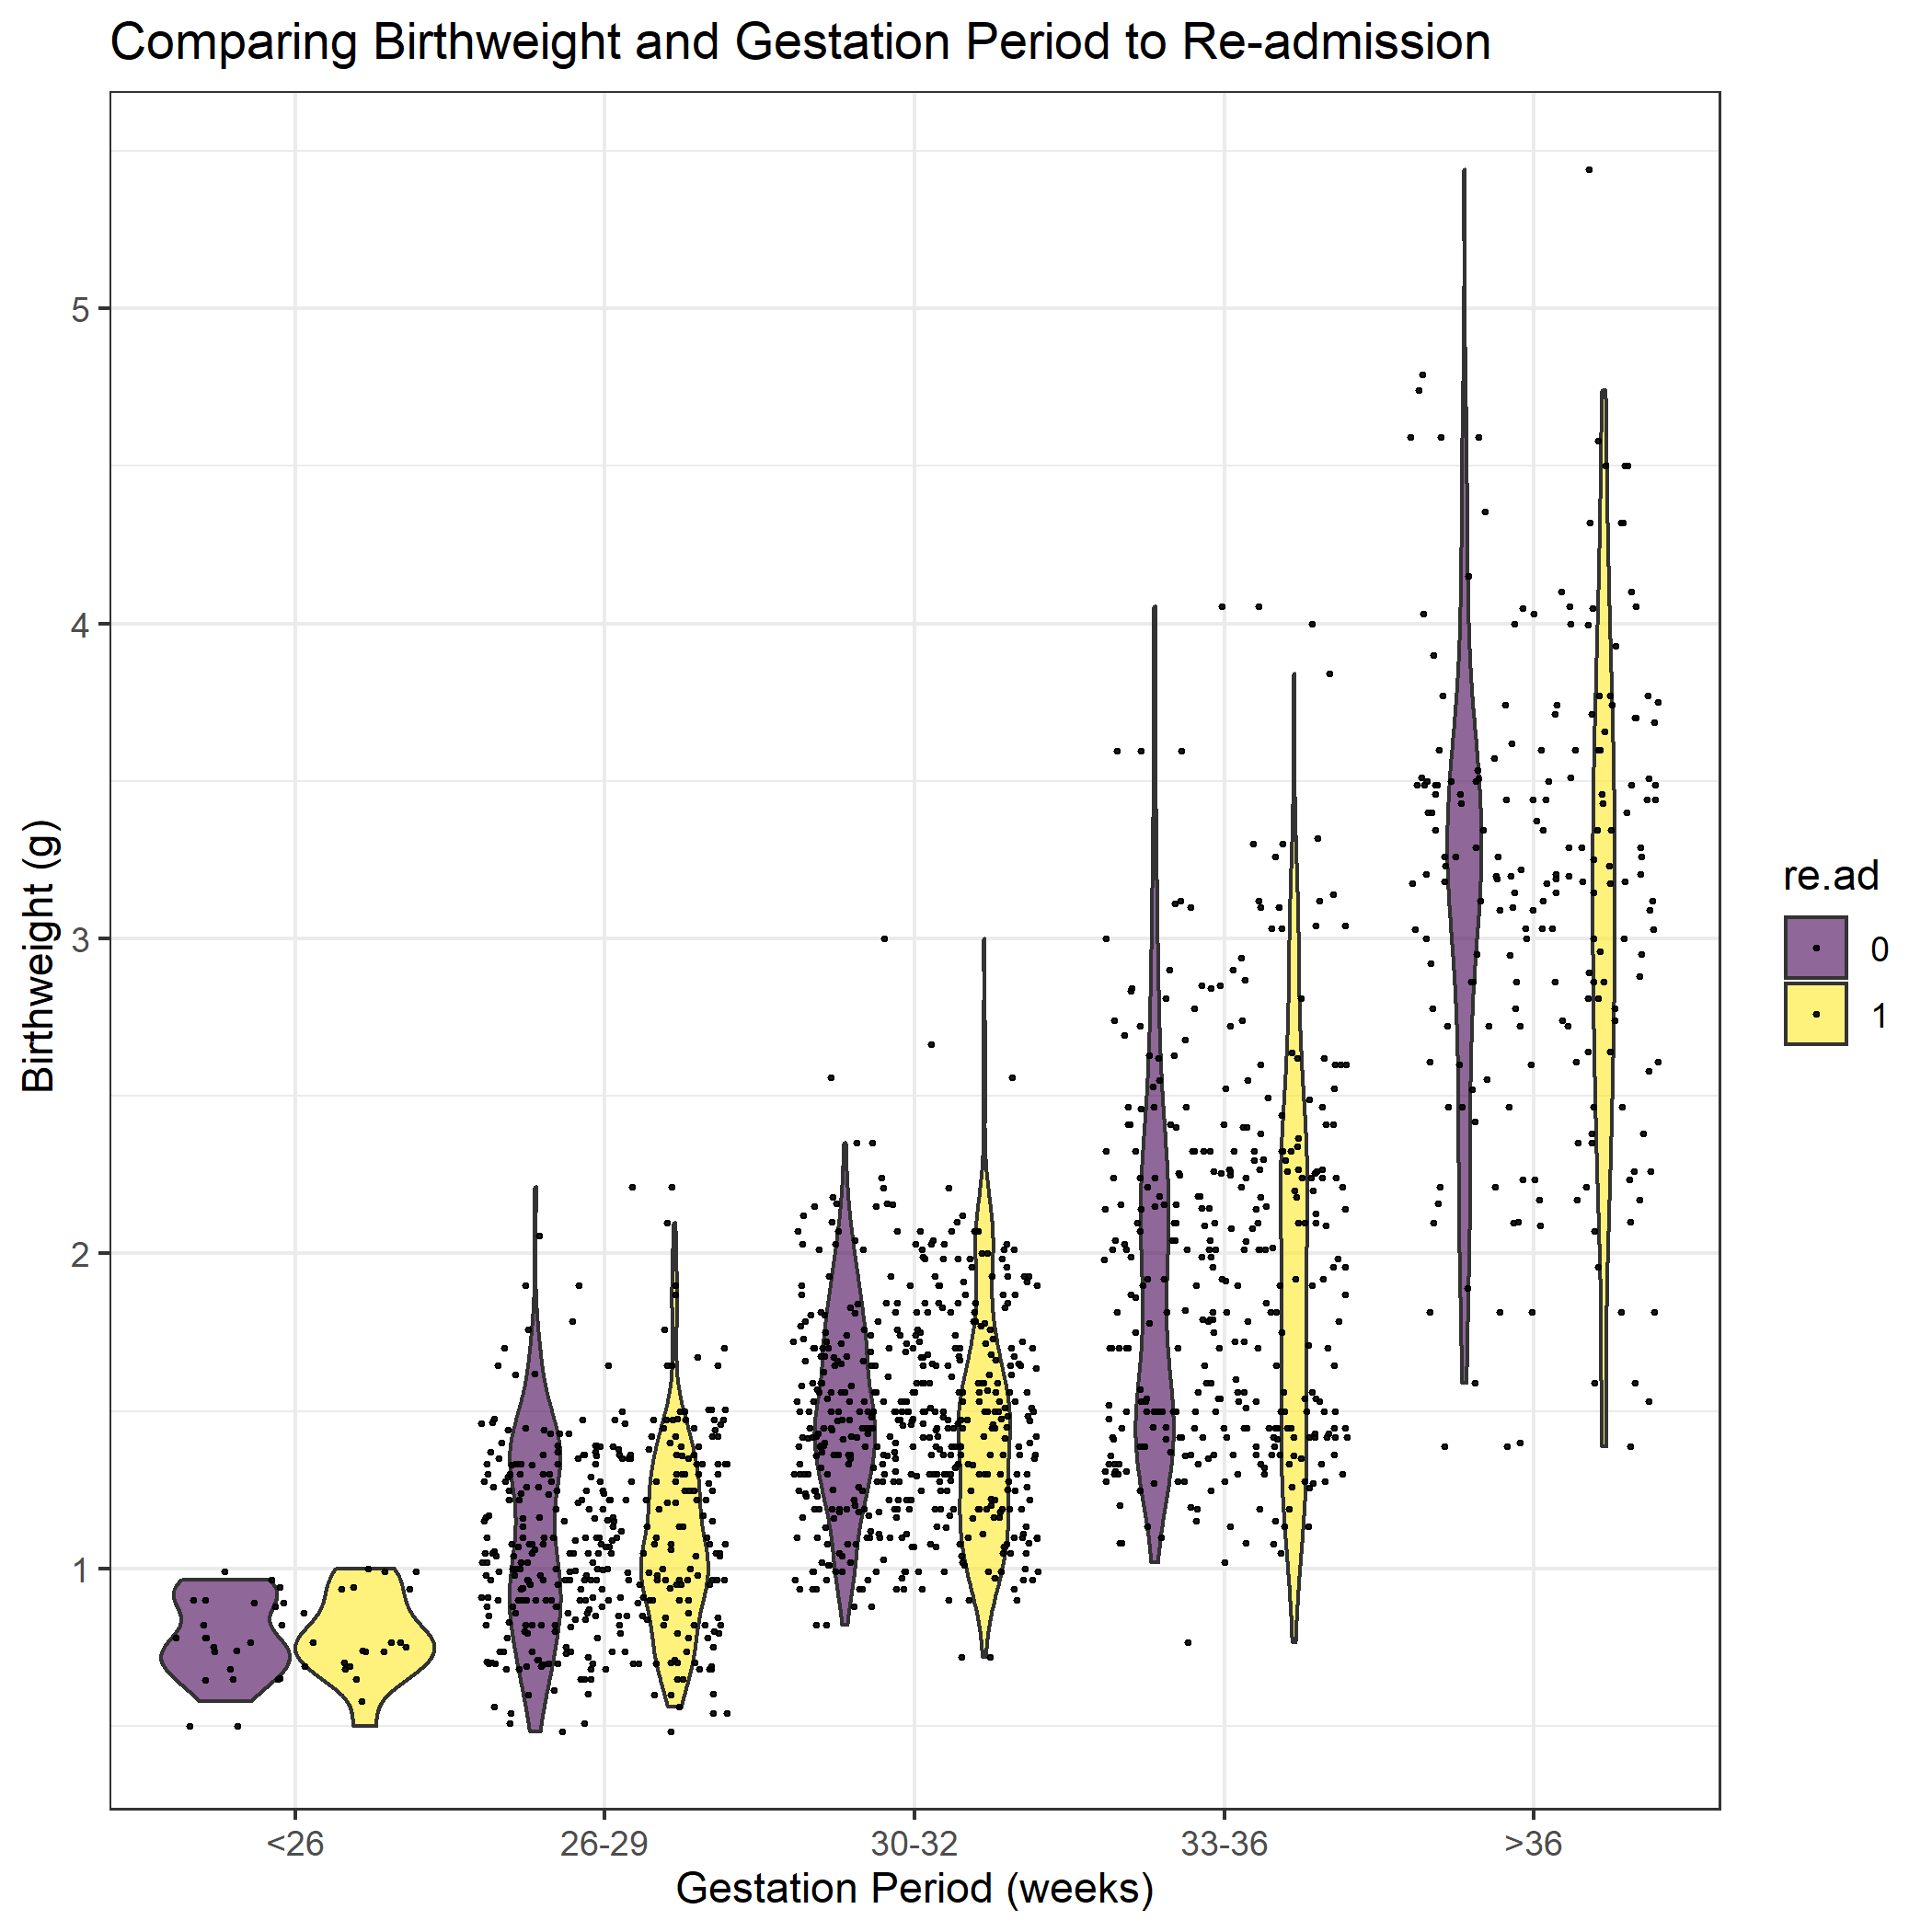
\includegraphics[width=0.4\textwidth]{images/bwt.gest.png}
    \caption{Gestation vs Birthweight for Re-admission. Purple - No readmission, Yellow - readmission}
    \label{img:bwt-gest}
\end{figure}

\begin{figure}[ht]%
    \centering
    \subfloat[\centering Birthweight and Gender vs Re-admission]{{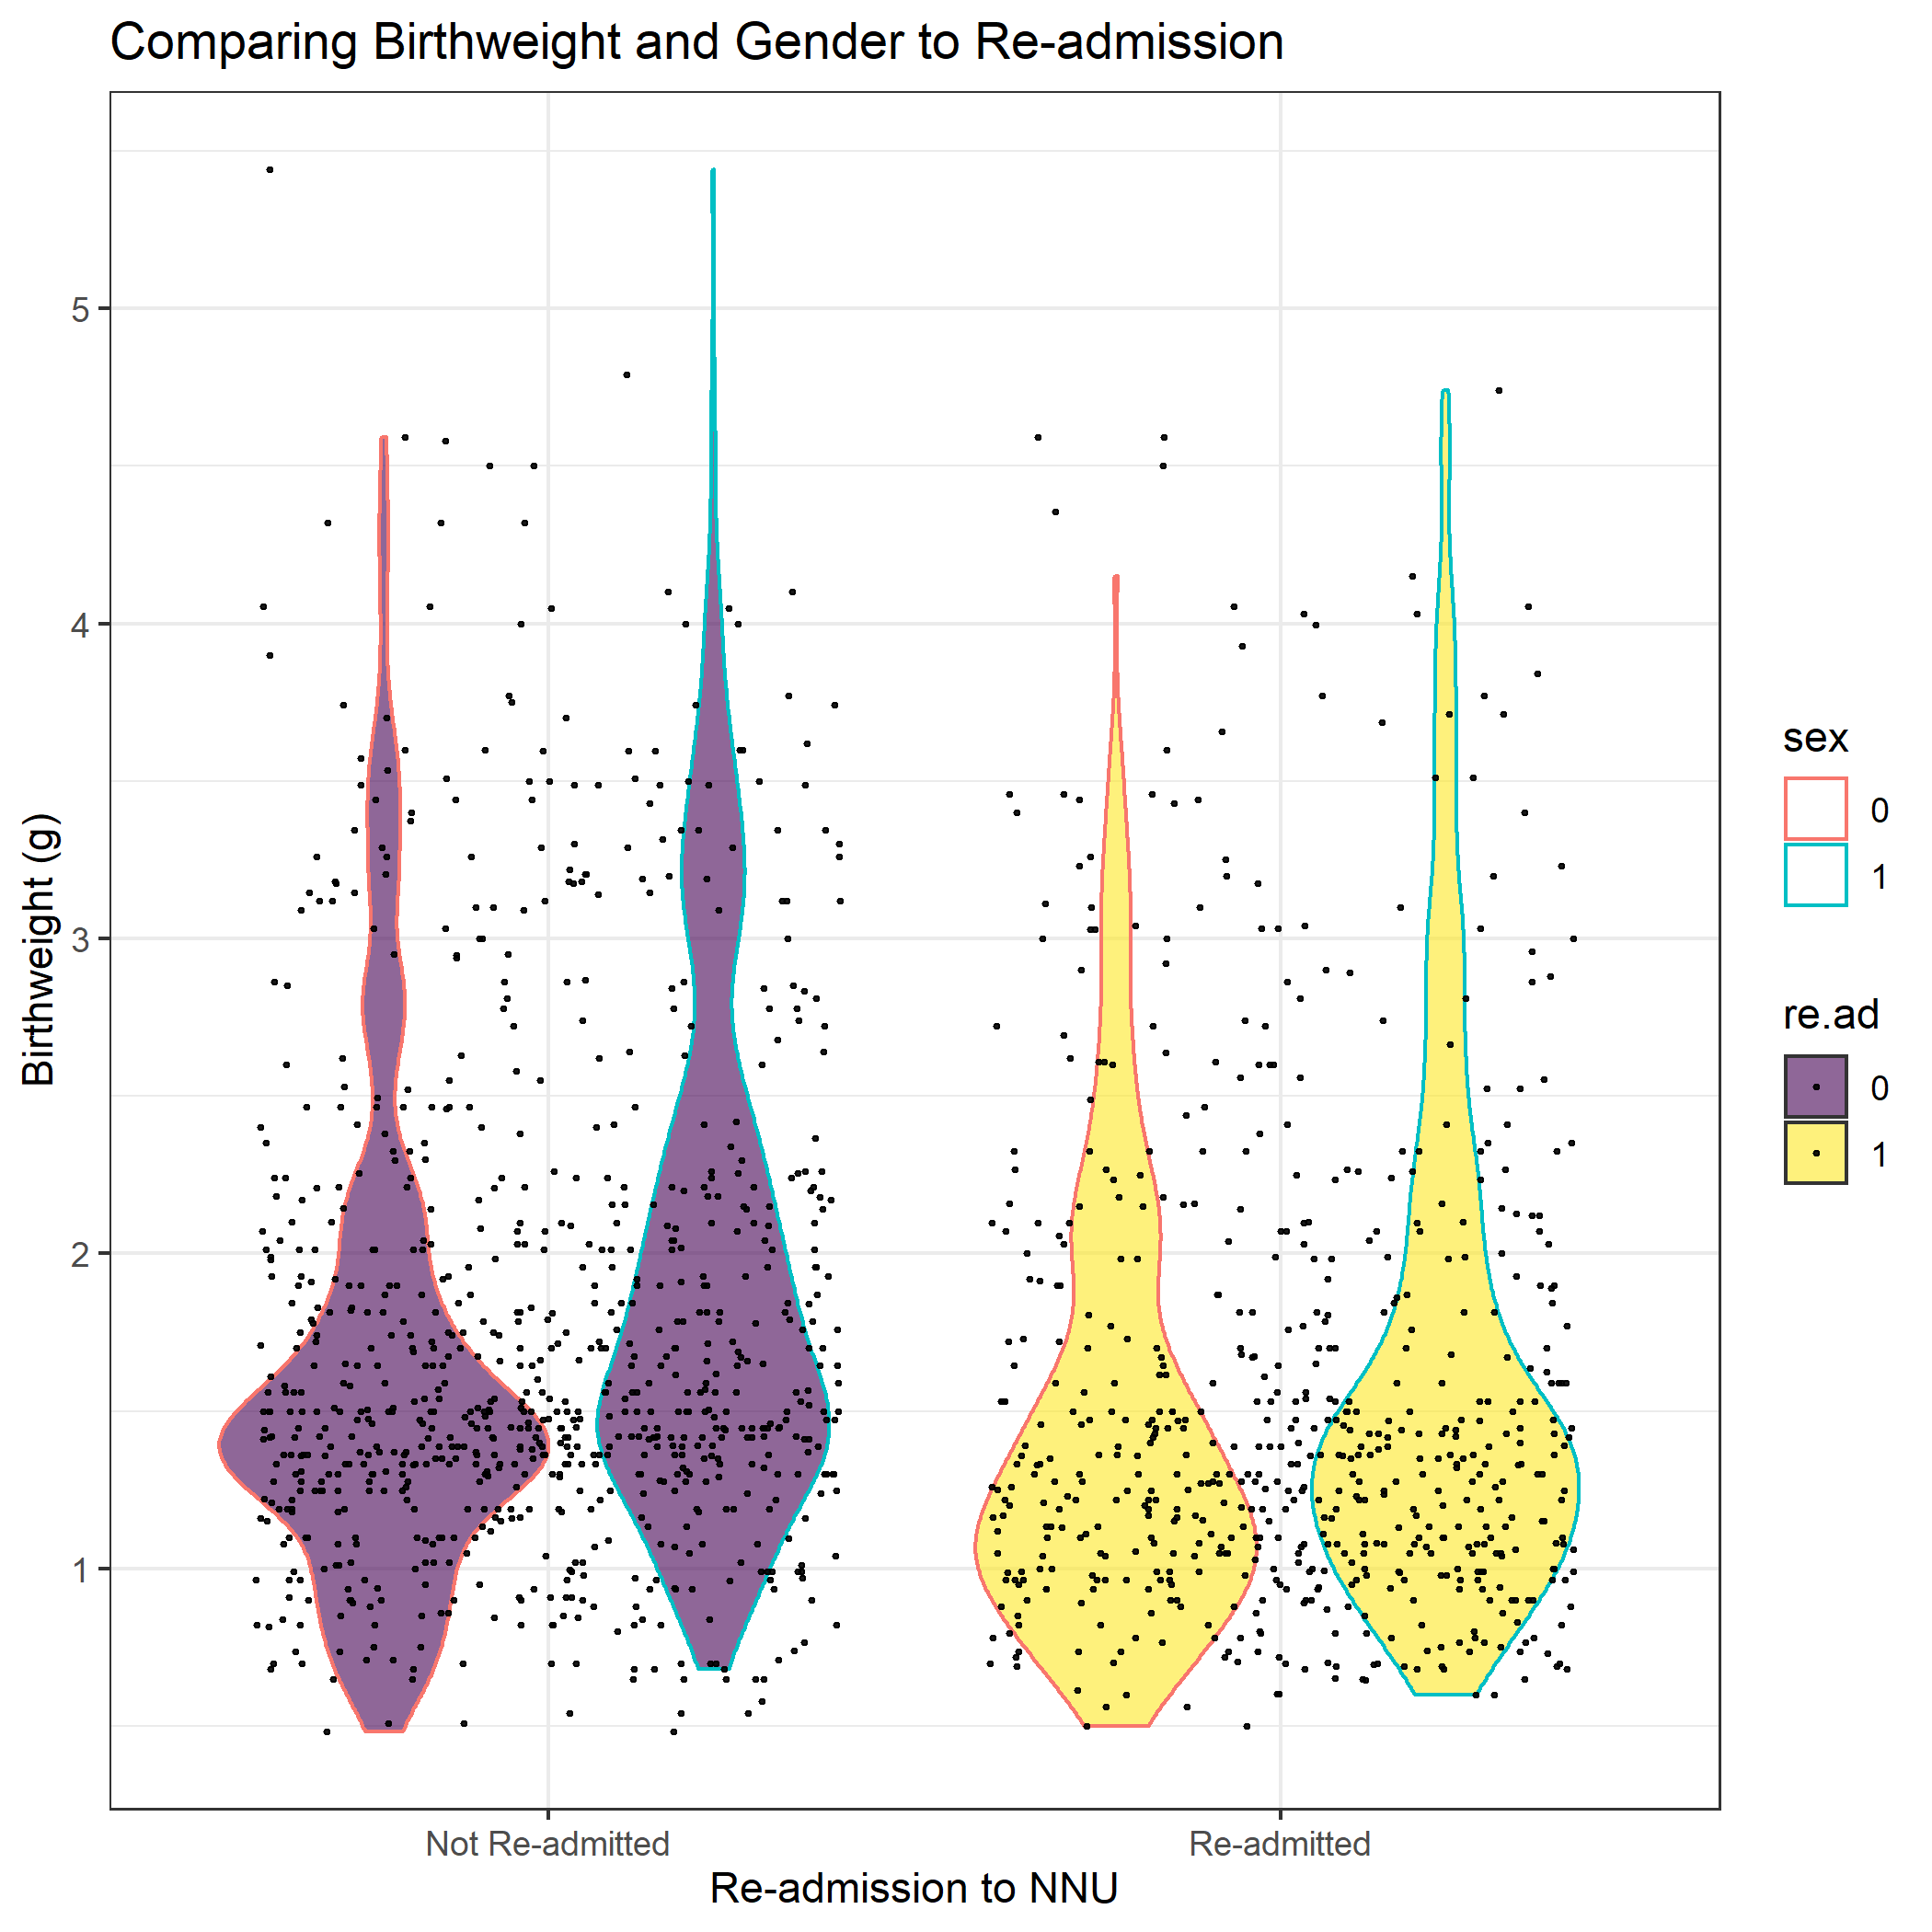
\includegraphics[width=0.4\textwidth]{images/bwt.gender.png} }}%
    \qquad
    \subfloat[\centering Length of Stay and Gender vs Re-admission]{{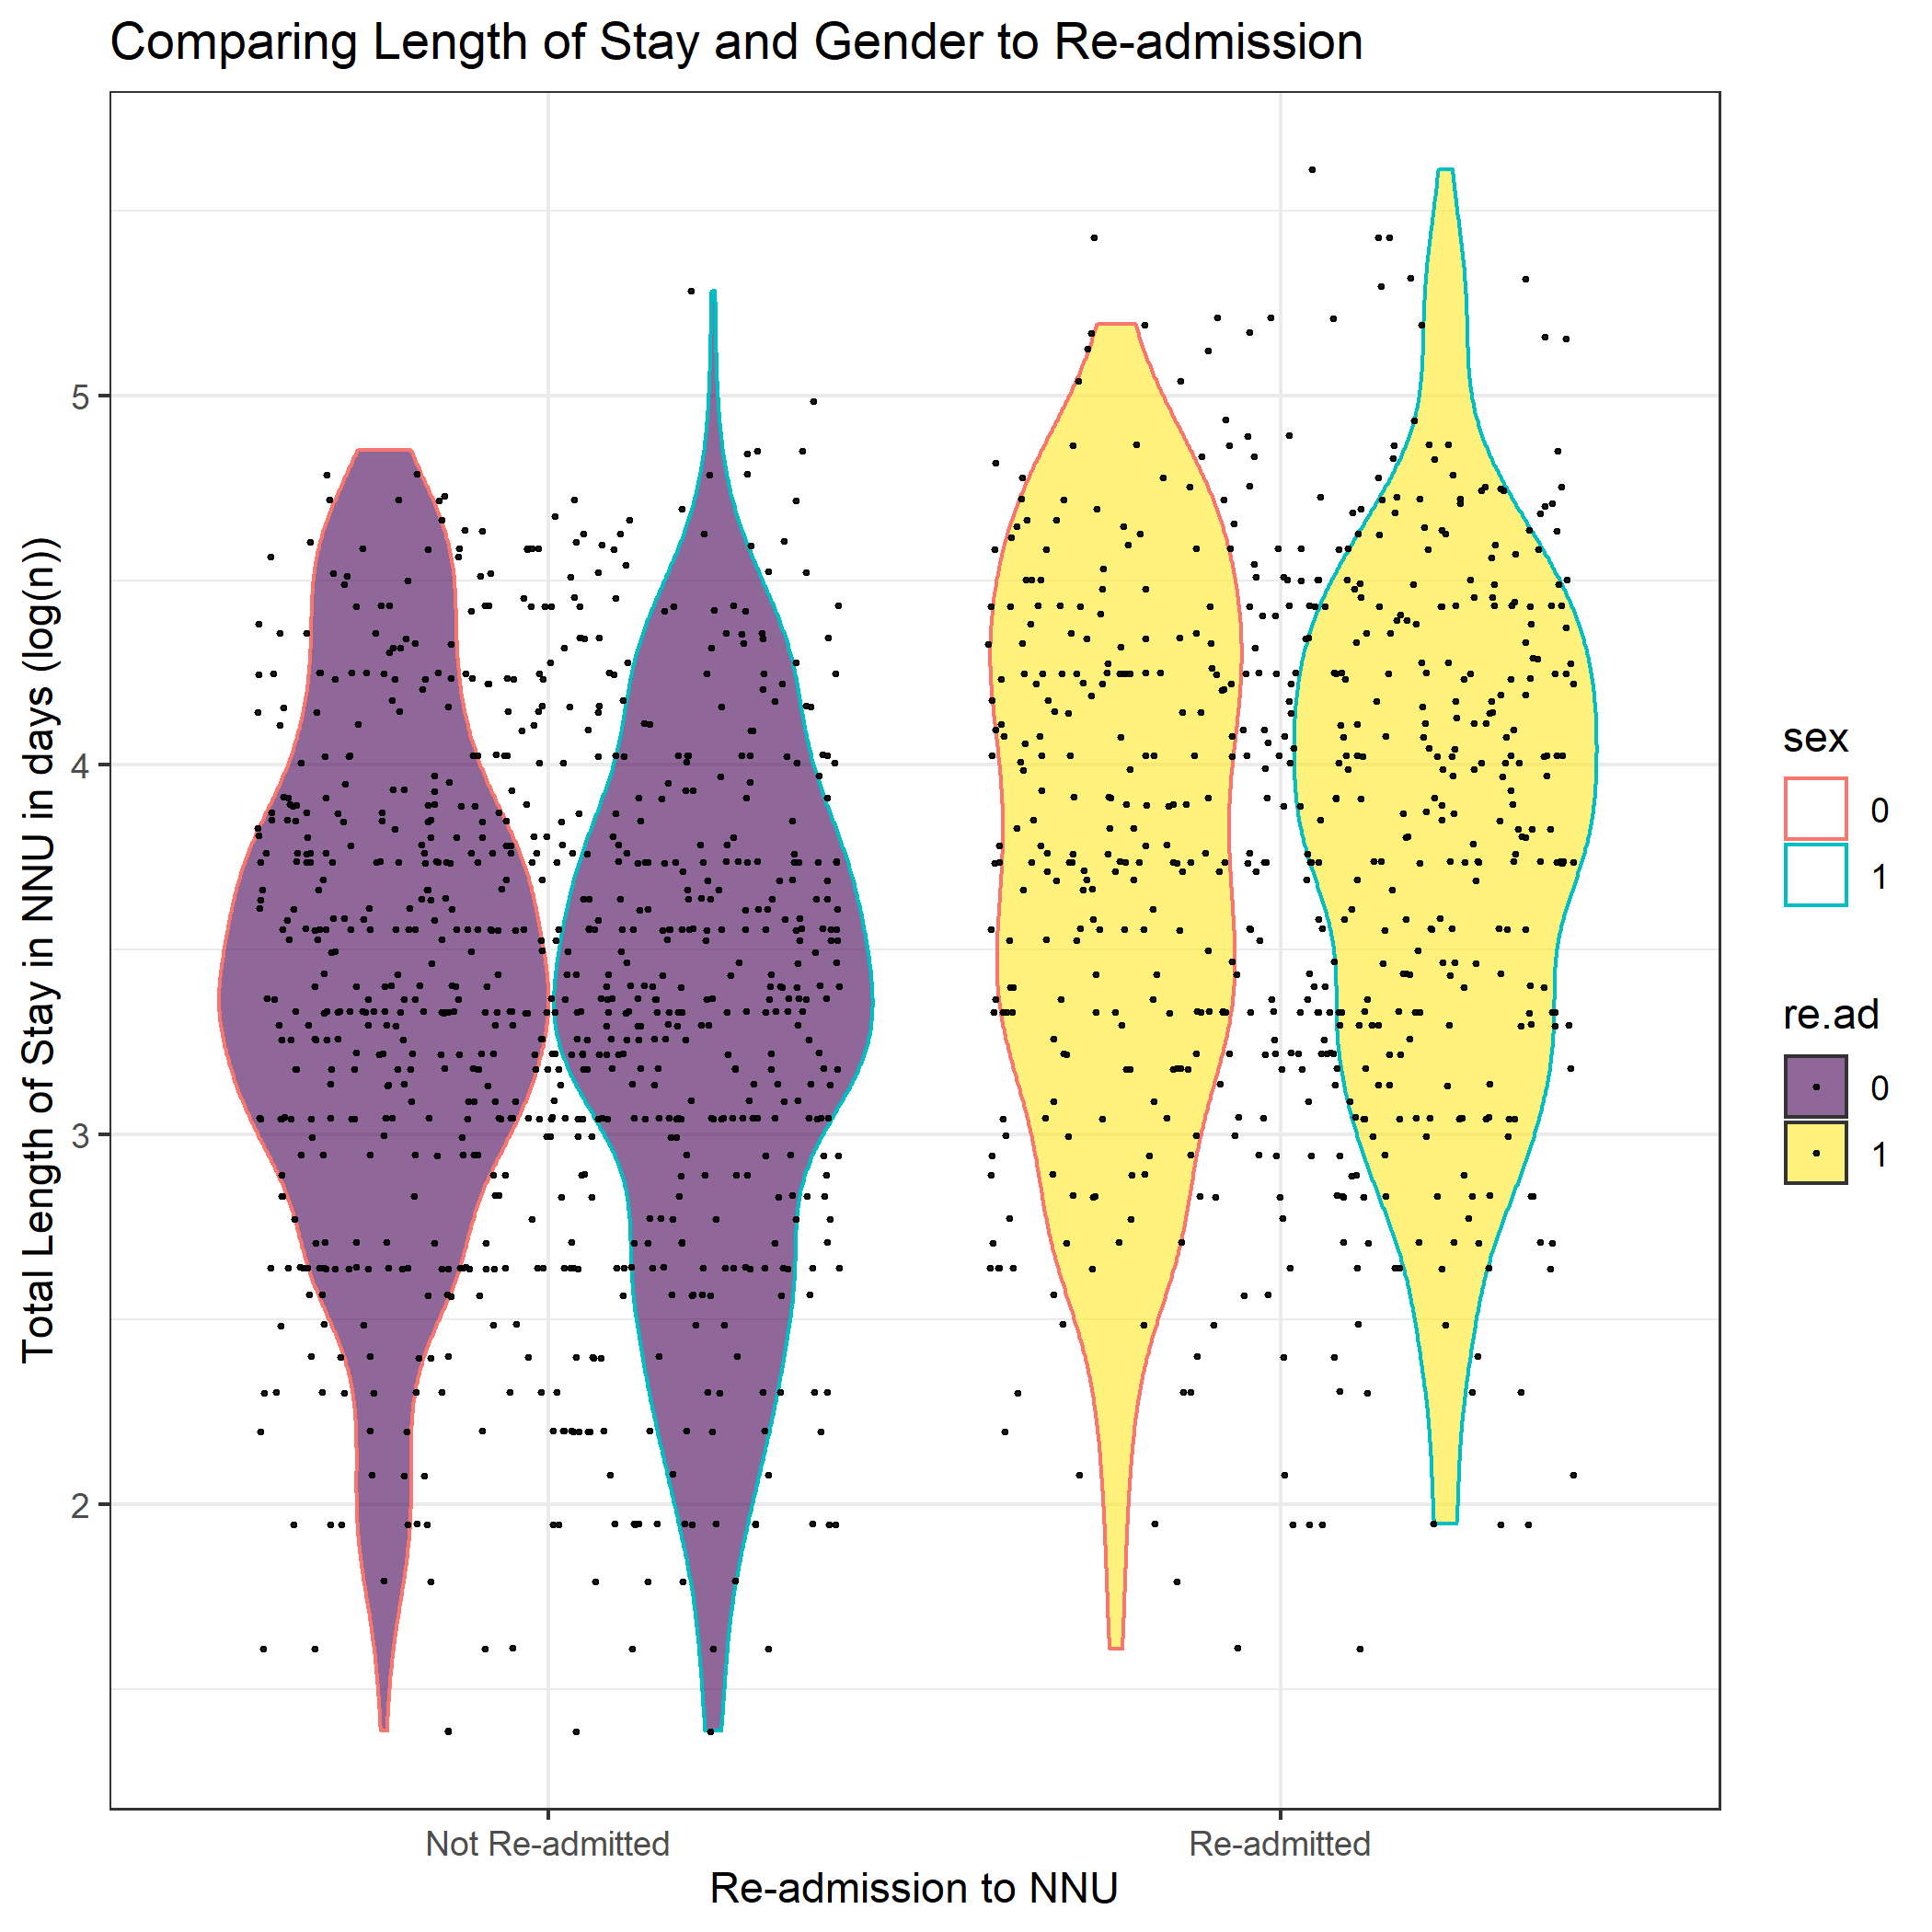
\includegraphics[width=0.4\textwidth]{images/los.gender.png} }}%
    \caption{Birthweight and Length of Stay with Gender vs Re-admission. Outline : Blue - Male, Pink - Female}%
    \label{fig:genders}%
\end{figure}

\begin{align}\label{eq:binom}
    &f(x,\pi) = \binom{n}{k} \pi^{x}(1-\pi)^{(n-x)} && x = 0,1,2,\dots,n. 
\end{align}
Using the binomial distribution (from Eq.\ref{eq:binom}), and factoring the quantitative variables to form into dummy matrices, as in Equation \ref{eq:arr}. Where $\textit{I}$ is the identity matrix.
\begin{equation}\label{eq:arr}
    X_{\text{gest}} =
        \begin{bmatrix}
            x_{1} & x_{2} & x_{3} & x_{4} & x_{5}
        \end{bmatrix} \Rightarrow X_{1488\times 5} = \textit{I}
\end{equation}

By creating an initial generalised linear model (GLM), based on the binomial distribution presented in Equation \ref{eq:binom}, which considers all variable interactions and transformations. Thus the `los` variable, total length of stay in hospital in $\log(\text{days})$ during the initial admission, is added into a secondary model to determine if these are identical. Which would prove how impactful the secondary post-birth response variable is on the overall model.

Knowing that `los` does have an impact when included as a covariate, the model needs to be checked for over-dispersion. The expected variance of the data samples from the binomial distribution is $\sigma^{2}=n\pi(1-\pi)$, where $n$ is the number of observations, $\pi$ is the probability of belonging the set $Y=1$. An over-discrepancy is defined as the observed variance of the response variable being greater than the expected variance of the binomial distribution. Over-dissociation can lead to seemingly bizarre standard error tests and imprecise significance tests. When over-dissociation occurs, the GLM function can still be used to fit the logistic regression, however the binomial distribution requires to be replaced by the Quasi-binomial Distribution. This can test for the occurrence of over-dispersion, if $\phi > 1$, it needs to be considered using quasi-likelihood. One way to detect an over-discrepancy is to compare the residual deviation of the binomial distribution model with the residual degrees of freedom if the ratio shown in Equation \ref{eq:phi}
\begin{equation}\label{eq:phi}
    \phi = \frac{\text{Residual Deviation}}{Residual DF}
\end{equation}
If $\phi > 2$, we can consider that there is an over-dispersion. Fitting the model twice, in addition to using quasi-binomial for the second model. 

The null hypothesis $H0: \phi = 1$ and alternative hypothesis $H1: \phi \ne 1$ can be tested by the provided p value. If P is very small (less than 0.05), we can reject the null hypothesis.

With both the forward and backward methods having obvious shortcomings, the forward not reflecting changes after the introduction of new independent variables, since the AIC corresponding to the regression equation is the minimum when introduced; the backward method has no chance to re-perform the regression equation, stepwise regression combines forward stepwise and backward stepswise. Whereby variables are entered one at a time, in each step it is re-evaluated, variables that do not contribute to the model are removed, and prediction variables may be added or deleted several times until the optimal model is obtained. Using ANOVA to compare the models, if there is no significant difference, we tend to use the stepwise regression model



%% SECTION RESULTS
\section{Results}\label{sec:results}
The GLM's described in Section \ref{sec:method}, the preliminary GLM with and without `los` are graphed in Figures \ref{img:glm-mod1-los} and \ref{img:glm-mod1-nolos}.

Comparing these two models using ANOVA, results in Table \ref{tab:anova-1}, it is clear that adding the `los` variable has a significant effect on the model and the interactions with other covariates.
\begin{figure}[ht]
    \centering
    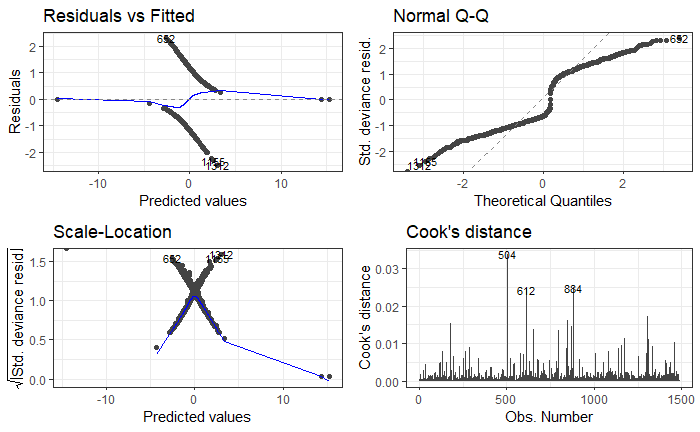
\includegraphics[width=0.7\textwidth]{images/mod.nolos.png}
    \caption{Preliminary GLM Model with 9 Covariates without `los`}
    \label{img:glm-mod1-nolos}
\end{figure}

\begin{figure}[ht]
    \centering
    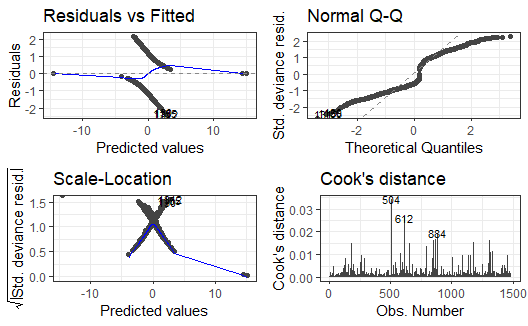
\includegraphics[width=0.7\textwidth]{images/mod.los.png}
    \caption{Preliminary GLM Model with 9 Covariates with `los`}
    \label{img:glm-mod1-los}
\end{figure}

\begin{table}[]
    \centering
    \begin{tabular}{|c|ccccc|}
        \hline
         & Residual DF & Residual Deviance & DF & Deviance & $P(>\chi)$ \\
        \hline
        1 & 1404 & 1722.7 &    &         &         \\
        2 & 1405 & 1768.7 & -1 & -46.068 & 0.0000  \\
        \hline
    \end{tabular}
    \caption{Anova Comparison of Binomial GLM with and without the secondary response variable `los`}
    \label{tab:anova-1}
\end{table}

Calculating $\phi$ from a binomial glm, using the formula in Eq.\ref{eq:binom}, $\phi = 1.254831$. Although $X>1$, it is still a small value, hence to quantitatively determine the analysis the p-value is calculated using a $\chi_1^2$ test on the quasi-binomial model. $P=0.4950646$, which is far larger than 0.05, as described in the null hypothesis, and therefore the quasi-binomial model can be used.

\begin{table}[]
    \centering
    \begin{tabular}{|c|ccccc|}
        \hline
         & Residual DF & Residual Deviance & DF & Deviance & $P(>\chi)$ \\
        \hline
        1 & 1472 & 1850.8 &    &         &         \\
        2 & 1452 & 1822.0 & 20 & 28.838 & 0.09101  \\
        \hline
    \end{tabular}
    \caption{Anova Comparison of the standard binomial GLM with the stepwise binomial}
    \label{tab:anova-2}
\end{table}

Using a stepwise regression model on the binomial GLM, in both directions attempting to reducing the AIC. ($\text{AIC}=1883$) and then performing an ANOVA test comparing the stepwise model with the original binomial, results in Table \ref{tab:anova-2}. Showing that $P=0.114 > 0.05$, which is not significant. Therefore it can be judged that the two models are not significantly different at 95\% confidence. The stepwise regression model is chosen to be the final model 

\begin{table}[ht]
    \centering
    \begin{tabular}{|c|cccc|}
        \hline
                     & Estimate    & Std. Error & Z Value & $P(>|Z|)$ \\
        \hline
                     & -2.92135    & 0.53208  & -5.490 & 4.01e-08 \\
        \hline
        cns1         & -0.77454    & 0.36077  & -2.147 &  0.03180 \\ 
        size1        &  1.23064    & 0.37916  &  3.246 &  0.00117 \\ 
        emp.f1       &  0.24307    & 0.35590  &  0.683 &  0.49463 \\   
        emp.m1       & -1.30891    & 0.56873  & -2.301 &  0.02137 \\ 
        edu2         & -0.44006    & 0.31121  & -1.414 &  0.15735 \\    
        edu3         &  0.12542    & 0.33830  &  0.371 &  0.71083 \\    
        edu4         & -0.21846    & 0.40323  & -0.542 &  0.58798 \\   
        los          &  0.76432    & 0.08051  &  9.493 &  < 2e-16 \\ 
        sex1         &  0.47432    & 0.11353  &  4.178 & 2.94e-05 \\ 
        accom1       & -0.44403    & 0.14160  & -3.136 &  0.00171 \\ 
        cns1:emp.f1  &  0.96974    & 0.38087  &  2.546 &  0.01089 \\
        size1:emp.f1 & -1.24017    & 0.40183  & -3.086 &  0.00203 \\ 
        emp.m1:edu2  &  1.39247    & 0.58795  &  2.368 &  0.01787 \\ 
        emp.m1:edu3  &  0.36251    & 0.61228  &  0.592 &  0.55381 \\    
        emp.m1:edu4  &  1.04384    & 0.66234  &  1.576 &  0.11503 \\ 
        \hline
    \end{tabular}
    \caption{Stepwise Binomial GLM Model Summary Results}
    \label{tab:stp-binom}
\end{table}
From Table \ref{tab:stp-binom}, mother employment (emp.f1) and mother education age (edu) have p-values larger than 0.05, which is not significant. All other coefficients of the covariates are deemed significant. Meanwhile the interaction of `emp.m1` and `edu2` have the greatest impact on the positive correlation of the model, and `emp.m1` has the greatest impact on the negative correlation on the model. As can be seen from the residual vs fitted plot in Figure \ref{img:glm-step-binom}, there is no systematic correlation between the residual and the fitted values, which means that we do not need to perform a response transformation of the independent variables. The normal Q-Q plot shows the probability plot of the standarised residuals for the values corresponding to the normal distribution, which can be seen that the model largely satisfies the assumption of normality. If the assumption of constant variance is met, then in the Scale-Location graph, the points around the horizontal should be randomly distributed. The graph does not seem to meet this assumption. And the cooks distance plot shows a no clear skew of data.

\begin{figure}[ht]
    \centering
    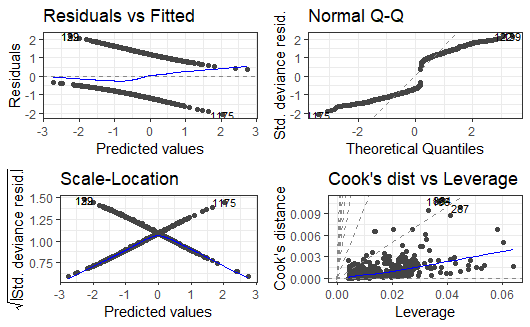
\includegraphics[width=0.7\textwidth]{images/mod.step.1.png}
    \caption{Stepwise Binomial GLM Model Summary Plots}
    \label{img:glm-step-binom}
\end{figure}

%% SECTION CONCLUSIONS
\section{Conclusions}\label{sec:conclusions}
In Section \ref{sec:results}, various models are discussed and compared in detail, resulting in the stepwise binomial being chosen as the superior model for accuracy. This model showed that a mothers employment and the age at which she leaves full-time education largely drove her child's re-admission to hospital within 12 months. As well as, the size of the NNU; larger NNU's led to a higher probability of readmission, where as smaller NNU's let to smaller probabilities. 

The model is good overall, but there are two shortcomings. Firstly, the model has high AIC values, which means that the fit is not very good. Secondly, there are insignificant coefficients in the model, which reduces the model's goodness-of-fit and the adjusted $R^2$

Further analysis of the data could include:
\begin{itemize}
    \item Comparing other distributions for model fit goodness, as aswell as covariate matching, perhaps also investing de-factorisation according to normal distributions of the data
    \item More data points is always helpful to get a bigger picture, perhaps scaling this data to more NNU centers would result in better analysis. The NNU's that form this dataset may be from lower income areas, perhaps NNU's in higher income areas see less admission, or deviate from the main outcome of this report.
\end{itemize}
\renewcommand\bibname{References}
\printbibliography

\end{document}

